\documentclass[titlepage]{article}

\usepackage[margin=1in]{geometry}
\usepackage{fancyhdr}
\usepackage{csquotes}
\usepackage{marginnote}
\usepackage{scrextend}
\usepackage[bottom]{footmisc}
\usepackage{enumitem}
\usepackage{amsmath,amssymb,amsthm}
\usepackage{mathtools,physics}
\usepackage{tikz}
\usepackage{pdfpages}
\usepackage[hidelinks]{hyperref}

\fancypagestyle{main}{
    \fancyhf{}
    \fancyhead[L]{\leftmark}
    \fancyhead[R]{MATH 16110}
    \fancyfoot[R]{Labalme \thepage}
}

\MakeOuterQuote{"}

\reversemarginpar

\deffootnotemark{\textsuperscript{\textup{[}\thefootnotemark\textup{]}}}
\deffootnote[2.1em]{0em}{0em}{\textsuperscript{\thefootnote}}

\setenumerate[itemize,3]{label={\scriptsize$\blacksquare$}}

\newtheorem{lemma}{Lemma}
\newtheorem{corollary}{Corollary}

\setcounter{secnumdepth}{0}

\newcommand{\N}{\mathbb{N}}

\title{MATH 16110 (Honors Calculus I IBL) Notes}
\author{Steven Labalme}

\begin{document}




\maketitle



\pagenumbering{roman}
\tableofcontents
\newpage



\pagenumbering{arabic}
\pagestyle{main}
\renewcommand{\sectionmark}[1]{\markboth{#1}{}}
\section{Introduction to Proofs}
\begin{itemize}
    \item \marginnote{9/27:}Note: These answers address the exercises on the following document.
    \item We will prove Lemma 4 (i) by contrapositive.
    \setcounter{lemma}{3}
    \begin{lemma}
        Let $x,y$ be positive integers. Then $xy$ is odd if and only if $x$ and $y$ are both odd.
        \begin{proof}
            We wish to prove that if $x$ and $y$ are not both odd, then $xy$ is not odd. In other words, we wish to prove that if at least one of $x$ or $y$ is even, then $xy$ is even. Let's begin. WLOG, let $x$ be even. Then $x=2k$ for some $k\in\N$. Thus, $xy=2(ky)$, proving that $xy$ is even since $ky\in\N$. The proof is symmetric for $y$.
        \end{proof}
    \end{lemma}
    \item We now prove Corollary 5.
    \setcounter{corollary}{4}
    \begin{corollary}
        Let $x,y$ be positive integers. Then $xy$ is even if and only if at least one of $x$ and $y$ is even.
        \begin{proof}
            We wish to prove that $xy$ is even if and only if at least one of $x$ and $y$ is even. Consequently, we must prove the dual implications "if $xy$ is even, then at least one of $x$ and $y$ is even" and "if at least one of $x$ and $y$ is even, then $xy$ is even." Let's begin. For the first statement, let $xy$ be even and suppose for the sake of contradiction that and both $x$ and $y$ are not even, i.e., are odd. But by Lemma 4, it follows from the assumption that $x$ and $y$ are both odd that $xy$ is odd, which contradicts the fact that $xy$ is even. Therefore, at least one of $x$ or $y$ must be even. As to the second statement, suppose that at least one of $x$ or $y$ is even. In this case, $x$ and $y$ are not both odd. Thus, by Lemma 4, $xy$ is not odd, or, equivalently, $xy$ is even.
        \end{proof}
    \end{corollary}
    \item Are there positive integers $m,n$ such that $m$ and $n$ have no common factors (other than 1) and $m^2=3n^2$? Either give an example or prove that no example is possible.
    \begin{proof}
        Let $m,n$ be relatively prime positive integers and suppose for the sake of contradiction that $m^2=3n^2$. We divide into two cases (the case where $n$ is even, and the case where $n$ is odd); we seek contradictions in both cases. First off, if $n$ is even, then $n=2k$ for some $k\in\N$. Thus, $3n^2=3(2k)^2=12k^2=2(6k^2)=m^2$, proving that $m^2$ is even since $6k^2\in\N$. By Corollary 5, this implies that $m$ is even. Therefore, since $m$ and $n$ are both even, they have a common factor, a contradiction. On the other hand, if $n$ is odd, then $n=2k+1$ for some $k\in\N$. Thus, $3n^2=3(2k+1)^2=12k^2+12k+3=2(6k^2+6k+1)+1=m^2$, proving that $m^2$ is odd since $6k^2+6k+1\in\N$. Thus, by Lemma 4, $m$ is odd. Consequently, $m=2l+1$ for some $l\in\N$, so $m^2=(2l+1)^2=4l^2+4l+1=12k^2+12k+3$, the last equality holding because we also have $m^2=3n^2=12k^2+12k+3$. This implies the following.
        \begin{align*}
            4l^2+4l+1 &= 12k^2+12k+3\\
            4l^2+4l &= 12k^2+12k+2\\
            2l^2+2l &= 6k^2+6k+1\\
            2(l^2+l) &= 2(3k^2+3k)+1
        \end{align*}
        Since $l^2+l$ and $3k^2+3k$ are both natural numbers, the above asserts that an odd number equals an even number, a contradiction. Hence, in both cases, we must have that $m^2\neq 3n^2$.
    \end{proof}
    \item Are there positive integers $m,n$ such that $m$ and $n$ have no common factors (other than 1) and $m^2=6n^2$? Either give an example or prove that no example is possible.
    \begin{proof}
        Let $m,n\in\N$ have no common factors (other than 1), and suppose for the sake of contradiction that $m^2=6n^2$. Since $m^2=6n^2=2(3n^2)$, $m^2$ is even. It follows by Corollary 5 that $m$ is even, implying that $m=2k$ for some $k\in\N$. Thus, $6n^2=m^2=(2k)^2=4k^2$, so $3n^2=2k^2$. Since $k^2\in\N$, $3n^2$ is even. Consequently, we have that $n^2$ is even by Corollary 5 (since at least one of 3 or $n^2$ is even and $3=2(1)+1$ is odd). By Corollary 5 again, $n$ is even. Thus, $m$ and $n$ are both even, contradicting the assumption that they have no common factors other than 1.
    \end{proof}
    \item Are there positive integers $m,n$ such that $m$ and $n$ have no common factors (other than 1) and $m^2=4n^2$? Either give an example or prove that no example is possible.
    \begin{proof}
        Let $m=2$ and $n=1$. Then $m^2=2^2=4=4\cdot 1^2=4n^2$.
    \end{proof}
\end{itemize}

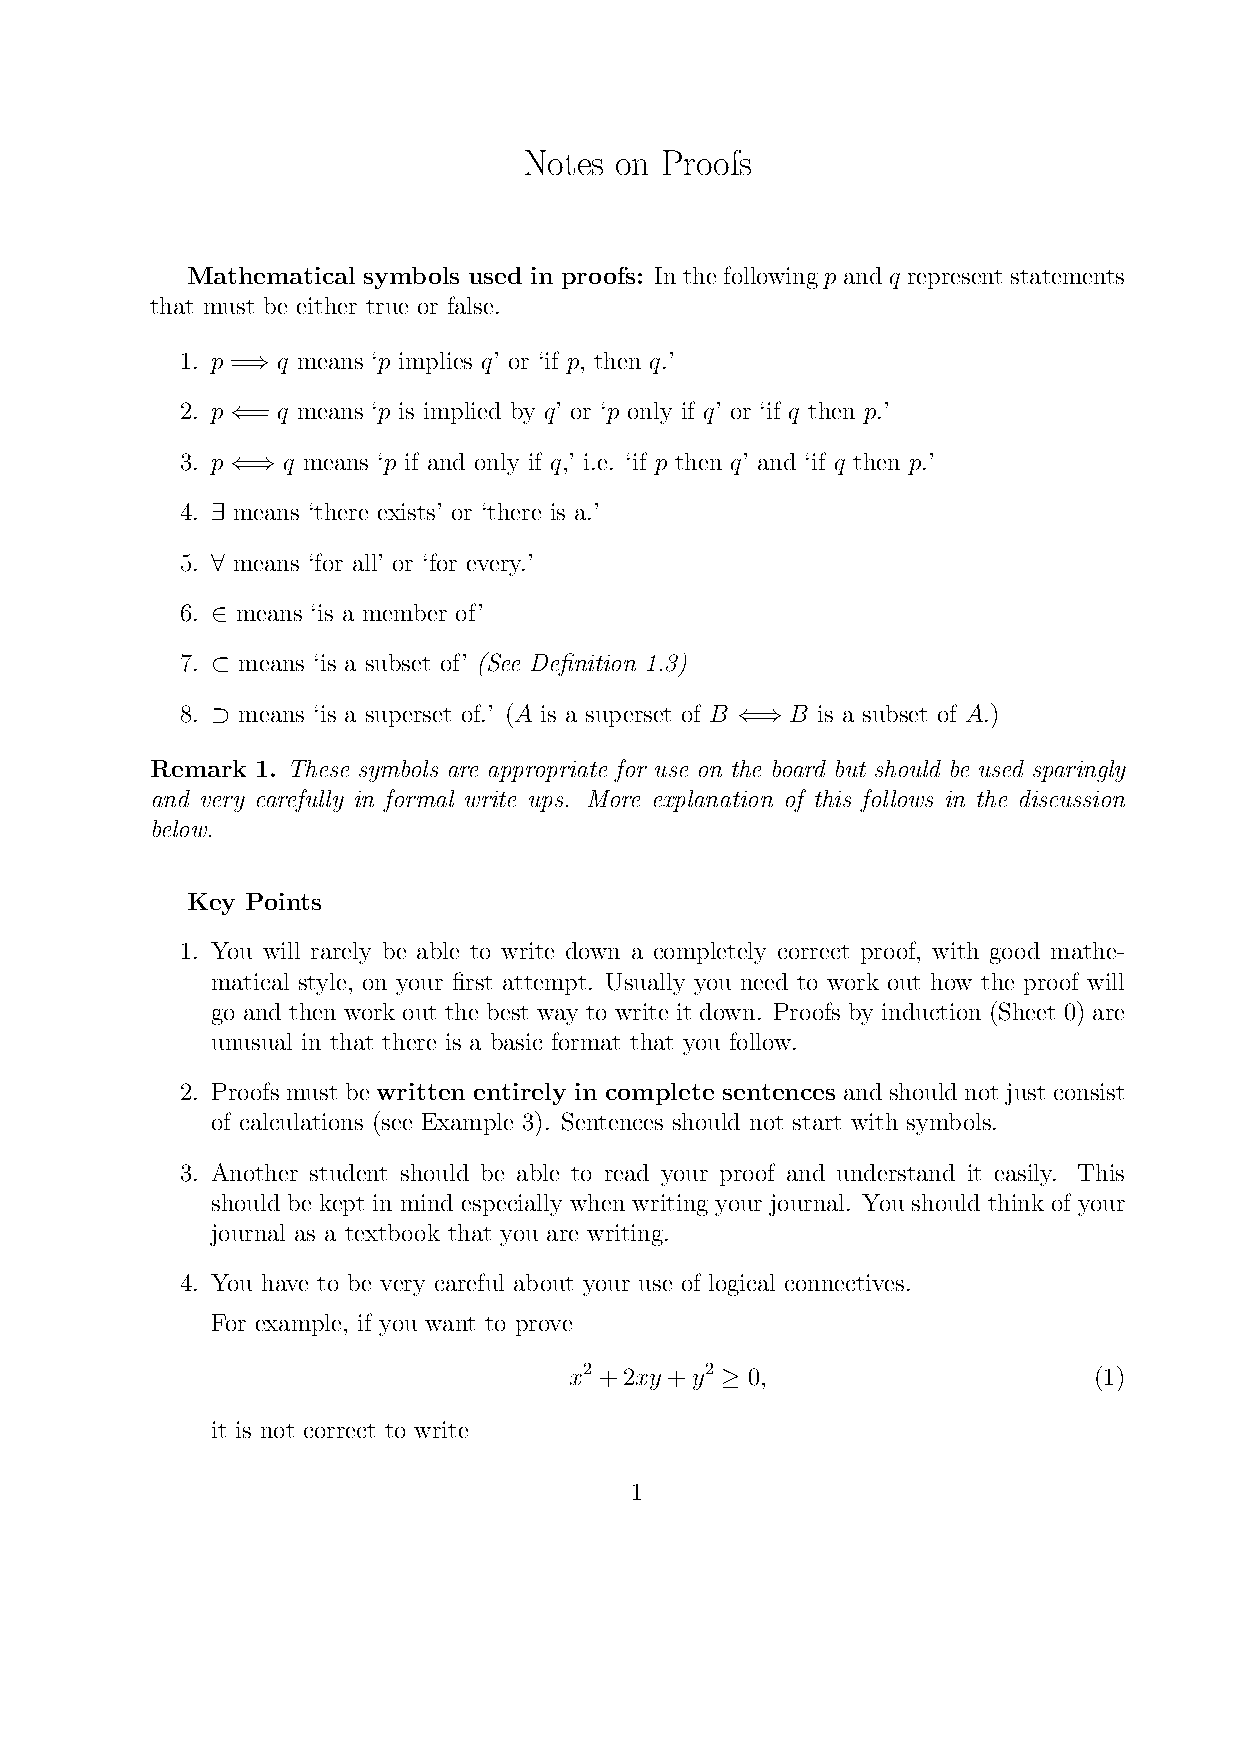
\includepdf[pages=-]{PDFs/WhatIsAMathematicalProof}



\section{Introduction to IBL}
\begin{itemize}
    \item \marginnote{9/29:}ZZ or zih-HWAY, Dixon Instructor in Department of Mathematics.
    \item Judson (super reader) is an advanced undergraduate who has taken this class before.
    \item Honors Calculus uses Spivak --- we do not have a textbook, just scripts!
    \begin{itemize}
        \item Few lectures in the traditional sense.
        \item Majority of material is presented and developed by the students.
        \item Several scripts will be covered throughout the quarter.
        \begin{itemize}
            \item In scripts: It is our job to complete the exercises, prove the theorems/lemmas/propositions, etc.
        \end{itemize}
        \item Be on the look-out for "\textcolor{green}{no proof required}" theorems.
        \item 3 chances to learn/review scripts material:
        \begin{enumerate}
            \item Before class, you prepare your own proof.
            \item During class, we discuss.
            \item After class and before the journal is due, we type up our own record of the proof in \LaTeX.
        \end{enumerate}
    \end{itemize}
    \item Before each class, she will tell us which theorems/exercises we need to work through.
    \item Your proofs do not have to be perfect in the beginning! Judson and ZZ will help us. Expect to present every other week.
    \begin{itemize}
        \item For the first two scripts, you have the ability to rewrite your journal after Judson reviews it to recover up to half of the lost credit.
        \item You only recover credit if your new solution is perfect.
        \item Return your changes one week after Judson grades it.
        \begin{itemize}
            \item Mark what parts/problems you have rewritten, and turn in the original as well.
        \end{itemize}
    \end{itemize}
    \item Later this afternoon, ZZ will share which Script 0 problems we should do before Thursday. Sign up for problems on a Google Sheet before 7:00 PM on Wednesday.
    \item She chooses a presenter based on our 0-3 rankings.
    \begin{itemize}
        \item A 0 means you don't know stuff or don't want to present.
        \item A 3 means you really want to present stuff.
        \item Other numbers are in between.
    \end{itemize}
    \item Class participation: When and how often and the quality of our presentations, and also how good are our questions that help presenters fill in the gaps.
    \item For hard proofs she may designate a backup presenter.
    \item We can use Overleaf for collaborative \LaTeX\ projects.
    \item We can check in with ZZ on our progress whenever throughout the quarter.
    \item She won't assign homework for the first week so that we can familiarize ourselves with \LaTeX.
    \begin{itemize}
        \item First HW assignment is due Thursday next week (10/8/2020)?
    \end{itemize}
    \item Judson's office hours: We get to talk to him one-on-one with questions.
    \begin{itemize}
        \item Problem session: we're all working collaboratively to figure something out.
    \end{itemize}
    \item You have one chance to ask for a 24-hour extension on HW (like if you're sick).
    \item In the case of a switch to virtual class:
    \begin{itemize}
        \item We can present by turning our phone into a document camera or using a white board behind us or typing up in \LaTeX\ (in real time?).
    \end{itemize}
    \item Get good at writing --- you cannot type up your solutions during exams!
    \item We submit HW assignments through Canvas if we type it up in \LaTeX, or in class by hand. It's nice if we can type it up.
\end{itemize}




\end{document}